\chapter{Web-Oberfläche für das IVS}
\label{ch:ivs}

Das erste größere Projekt war die Entwicklung einer Web-Oberfläche für ein bereits
bestehendes, jedoch noch nicht vollständiges Bildverarbeitungssystem. Sowohl Webinterface
als auch Bildverarbeitung waren bereits vorhanden, jedoch nicht für den aktuellen
Anwendungszweck geeignet und somit war eine Überarbeitung unabdingbar.

Die Aufgabe des betreffenden Systems ist die Ausrichtung einzelner Keramikseiten,
welche dann in weiteren Schritten verarbeitet werden. Dabei geht es um die Produktion
von Lambdasonden, wie sie in der Abgasfilterung von Autos zum Einsatz kommen.

Diese Keramik-``sheets'' werden dabei mit hochpräziser Genauigkeit ausgestanzt,
weswegen sie vor dem Stanzen entsprechend ausgerichtet werden müssen. Eine physikalische
Ausrichtung ist dabei so gut wie unmöglich, da die gewünschte Genauigkeit dabei
nicht erreicht werden kann.

Das von isys entwickelte System erkennt nun mithilfe
zweier Kameras die Lage zweier Marken auf dem Sheet und somit die Lage auf dem verschieb-
und rotierbaren Tisch. Mithilfe der Bildverarbeitungssoftware wird nun eine Motorbewegung
errechnet, welche eine Ausrichtung des Werkstücks bewirkt. Anschließend kann das
Teil durch weitere Maschinen in seiner nun festgelegten Position weiterverarbeitet
werden.

Die Software besteht dabei nun aus drei verschiedenen Komponenten:
\begin{itemize}
	\item Dem \textit{ScbDrv}, welcher für die Ansteuerung der Motoren und Hardware
	verantwortlich ist.
	\item Dem \textit{IVS} (Isys Vision Server), welcher für die Auswertung der Kameradaten
	sowie die Bildverarbeitung und Errechnung der Endposition verantwortlich ist.
	\item Dem \textit{Webinterface}, welches dem Endkunden eine Möglichkeit zur Einsicht
	des aktuellen Status sowie zur Kontrolle über die Maschine gibt.
\end{itemize}

Während der ScbDrv nur geringfügig an die neue Maschinenkonfiguration angepasst
werden musste, war mein Betreuer mit der Anpassung des IVS an die neuen Marken (in
diesem Fall die Ecken der Keramiksheets) beschäftigt. Meine Aufgabe bestand aus
dem visuellen Redesign der Weboberfläche, dem Anpassen des Inhaltes (Entfernen überflüssiger
Elemente, Hinzufügen von neuen, wichtigen Dingen) sowie der Anpassung der Funktionalität
mithilfe von HTML, CSS und JavaScript.



\section{Einlesen in vorhandenen Code und Redesign}
\label{sec:ivs-einlesen}

Da das Interface auf der alten, bereits vorhandenen Version aufbauen sollte, war
das Einarbeiten in bereits vorhandenen Code notwendig. Um Änderungen vorzunehmen,
war dabei ein großes Verständnis für diesen Code nötig, da es sich um komplexe und
vor allem abstrakte Abläufe handelte, die nicht leicht nachzuvollziehen waren.


\subsection{Flat-Design mithilfe von CSS}
\label{subsec:ivs-einlesen-css}

Da meine bisherigen Erfahrungen mit Javascript und jQuery mittelmäßig bis wenig
vorhanden waren, machte ich mir zunächst das grafische Redesign der Webseite zur
Aufgabe. Mit CSS hatte ich bereits gearbeitet, sodass ich mich verhältnismäßig schnell
in das vorhandene Stylesheet einarbeiten konnte und erste Änderungen vornahm.

Dazu gehörten beispielsweise das Entfernen von Schatten (\texttt{box-shadow}),
die Anpassung von Farben oder das Ersetzen von Hintergrundbildern. Durch bereits
wenige Änderungen im Stylesheet konnte ich hierbei recht große Erfolge erzielen,
was die Modernität der Seite angeht.

\begin{figure}[H]
	\begin{minipage}{0.5\textwidth}
		\centering
		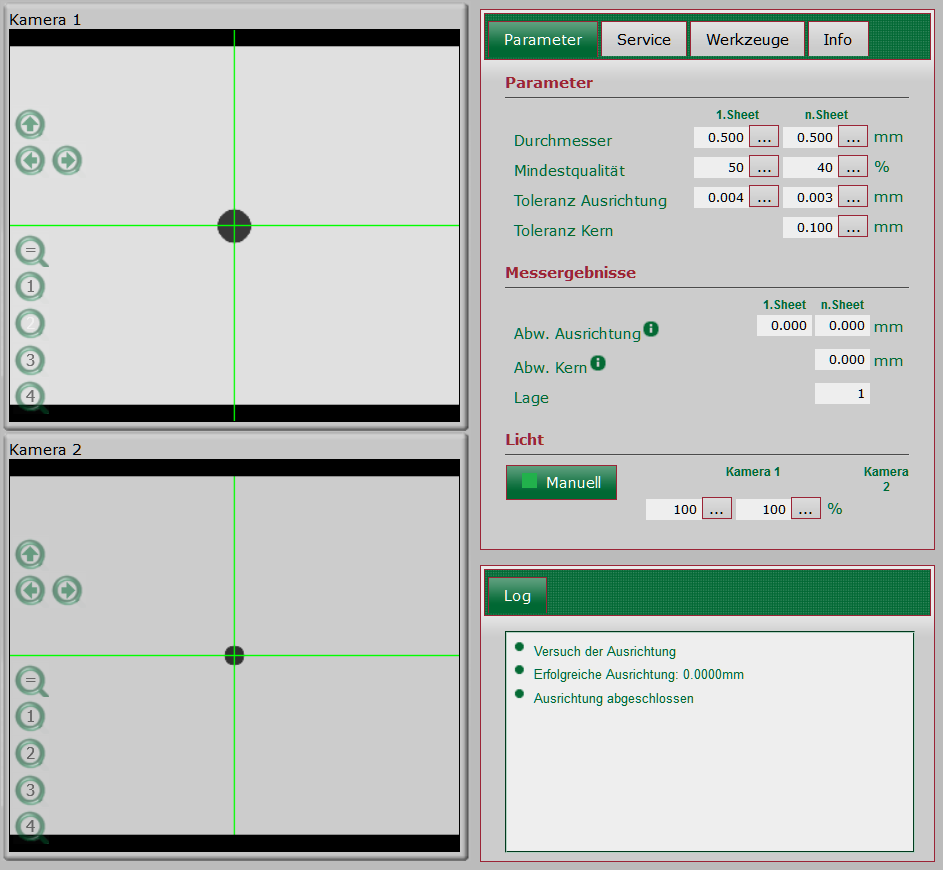
\includegraphics[width=\textwidth, height=\textwidth]{media/webinterface-alt.png}
		\caption{Interface vor dem Redesign}
		\label{fig:ivs-webinterface-alt}
	\end{minipage}
	\begin{minipage}{0.5\textwidth}
		\centering
		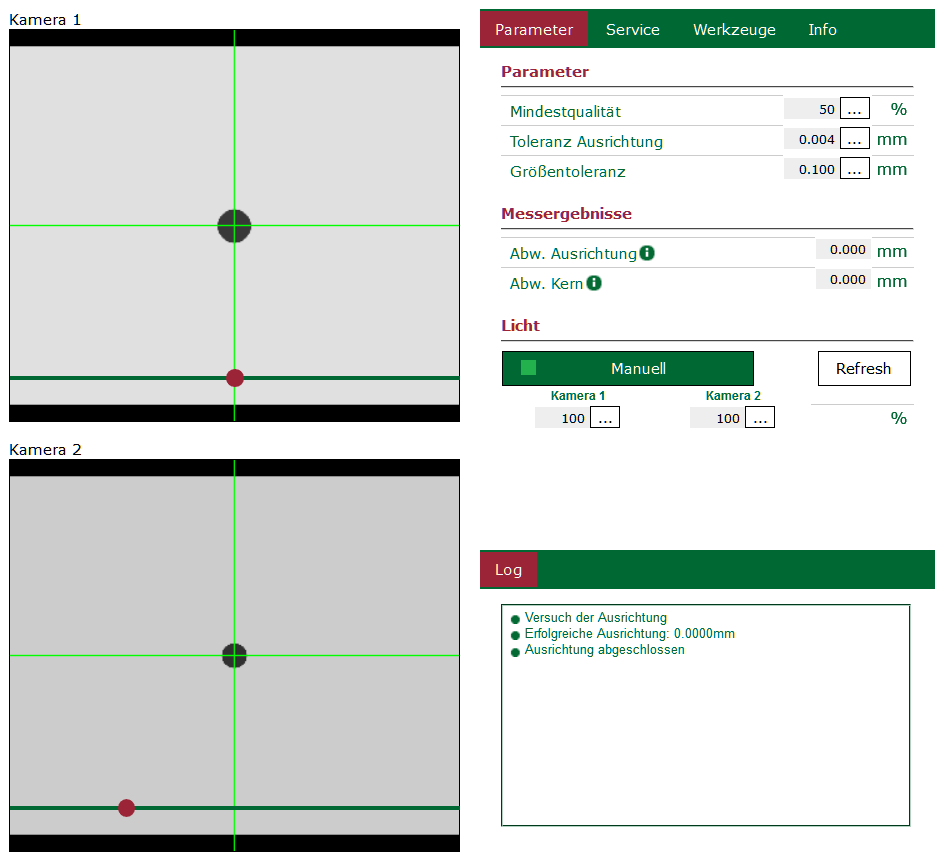
\includegraphics[width=\textwidth, height=\textwidth]{media/webinterface.png}
		\caption{Interface nach dem Redesign}
		\label{fig:ivs-webinterface}
	\end{minipage}
\end{figure}

\subsection{Javascript-Framework}
\label{subsec:ivs-einlesen-javascript}

In der bereits vorhandenen Version der Webseite wurde sämtliche Funktionalität durch
ein Javascript-Framework geregelt, welches unabhängig von Inhalt und Design steht.
Im Folgenden ging es nun darum, den hier geschriebenen Code durchzugehen, zu verinnerlichen
und zu verstehen.

Aufgrund der trotz weniger Codezeilen doch sehr hohen Komplexität und vor allem
den fehlenden Kommentaren gestaltete es sich als sehr schwierig, sich einzuarbeiten.
Ein weiterer Nachteil war meine mangelnde Erfahrung mit Javascript; durch viel Recherche
und weiterführende Beispiele konnte ich mir jedoch einiges herleiten und somit verstehen.

Weitere Modifikationen am Framework umfassten vor allem die Vereinfachung und Lesbarkeit
des Codes. Die Hauptaufgabe in dieser Phase war das Verständnis, da dies die Grundlage
für weitere Arbeit am Javascript war.



\section{Dokumentation des Frameworks}
\label{sec:ivs-dokumentation}

Eine weitere wichtige Aufgabe war das Dokumentieren des bereits vorhandenen Codes.
Da der ursprüngliche Autor leider nicht mehr bei isys vision angestellt war und
ich mich nun schon länger damit auseinandergesetzt hatte, sollte nun eine umfassende
Dokumentation des Aufbaus erstellt werden.

Dies erleichtert einerseits die Arbeit am Framework selbst (Änderungen und Updates
beispielsweise) und bietet denjenigen, die es nur verwenden (z.B. für eine neue
Webseite mit demselben Framework), ein einfaches, gut verständliches Interface. Weiterhin
können komplexere Vorgänge wie die Datenübertragung anschaulich erklärt und mithilfe
von Diagrammen verdeutlicht werden.


\subsection{Codekommentierung mit JSDoc}
\label{subsec:ivs-dokumentation-jsdoc}

Im ersten Schritt arbeitete ich dabei nur am Quelltext selbst, den ich zuvor schon
in lesbare Form gebracht hatte. Durch zusätzliche Kommentare an wichtigen und irreführenden
Stellen konnte ich dabei eine erste Grundlage schaffen. Die größte Änderung war
die Einführung einer Codedokumentation im \texttt{JSDoc}-Format\footnote{\url{https://en.wikipedia.org/wiki/JSDoc}},
ähnlich zu den bei Java eingesetzten JavaDoc-Kommentaren. Die Vorteile davon liegen
auf der Hand: Jede Methode bzw. Funktion hat somit eine eigene Beschreibung, in
der Funktionsweise, Parameter, Rückgabewert usw. beschrieben werden.

Ein weiterer Vorteil von JSDoc ist die Möglichkeit, die Dokumentation automatisch
zu generieren. Dies ist mit dem JSDoc-Tool von \texttt{Node.js} möglich, was nach
der Installation einfach über den Befehl \texttt{jsdoc file.js} aufgerufen werden kann.
Somit wird ein gut strukturiertes Dokument (inklusive Referenzen) automatisch erstellt.


\subsection{Beschreibung der API}
\label{subsec:ivs-dokumentation-beschreibung}

Nachdem der Quellcode selbst dokumentiert war, konnte ich mich nun mit den internen
Abläufen des Frameworks beschäftigen und diese anhand von Grafiken anschaulich machen.
In diesem Fall ging es vor allem um die Daten- und Befehlsübertragung vom IVS zum
Webinterface und umgekehrt.

Die Übertragung der Daten erfolgt hierbei über eine \texttt{XMLHttpRequest}, bzw.
(bei älteren Browsern) über ein \texttt{ActiveXObject}. Die Befehlscodes sind dabei
im HTML-Code der betreffenden Buttons gespeichert:

\begin{code}[language=html, caption={Ins HTML eingebettete Befehle für das IVS}, label={lst:ivs-html-befehle}]
<input type="text" size="6" maxlength="6" name="lms/SheetF.MinQuality">
<button name="lms/Cmd" value="10">Ausrichtung</button>
<button name="lms/Cmd" value="20">
	<ul>
		<li>LmsScb/Mot.RefOk</li>
		<li>Referenzfahrt</li>
	</ul>
</button>
\end{code}

In Zeile 1 wird beispielsweise das Register \texttt{lms/SheetF.MinQuality} geschrieben
und auf einen sechsstelligen Wert gesetzt, der vom Nutzer eingegeben wird.\\
In Zeile 2 befindet sich ein einfacher Befehlsbutton, der den Wert \texttt{10} ins
Register \texttt{lms/Cmd} schreibt (beim IVS ist dies der Code für eine Ausrichtung).\\
In den Zeilen 3 - 8 findet sich nun ein Knopf mit Status, der
\begin{itemize}
	\item den Wert \texttt{20} ins Register \texttt{lms/Cmd} schreibt und somit eine
	Referenzfahrt auslöst
	\item innerhalb der unsortierten Liste (Zeile 5) den Wert \texttt{LmsScb/Mot.RefOk}
	liest (Status der Referenzfahrt).
\end{itemize}
Die Liste (\texttt{<ul>}) dient dabei ausschließlich der Darstellung und hat keine
Auswirkung auf die Funktion; die Listenelemente werden innerhalb des Buttons entsprechend
formatiert. Weiterhin wird je nachdem, was im gelesenen Register \texttt{LmsScb/Mot.RefOk}
steht, ein entsprechendes Label gesetzt (grün falls Referenzfahrt OK, rot falls
nicht).

Im Javascript-Framework wird nun ein Event-Listener für alle Buttons und Eingabefelder
erstellt, der dann die entsprechenden Befehle erkennt. Diese werden in Form einer
URL in einer Liste gespeichert, welche dann mithilfe der bereits genannten \texttt{XMLHttpRequest}
bzw. des \texttt{ActiveXObject}s ans IVS gesendet werden. Die Antwort des IVS wird
dann entsprechend weiterverarbeitet und beispielsweise in Form eines Kamerabildes
direkt ausgegeben.


